% CVPR 2027 submission draft. Template: https://github.com/cvpr-org/author-kit
\documentclass[10pt,twocolumn,letterpaper]{article}

\usepackage[review]{cvpr}
%% This file contains a number of tweaks that are typically applied to the main document.
%% They are not enabled by default, but can be enabled by uncommenting the relevant lines.


%%
%% Official support for 2-column teaser figure
%%
\usepackage{cuted} %< for strip environment

%%
%% For auto-referencing of figures (see fig/teaser.tex and \label{} therein) 
%%
\usepackage{currfile} %< for \currfilebase macro

%%
%% caption and (global) spacing overrides
%%
\usepackage{caption} %< for "\captionof" commands (teaser)
% \setlength{\abovecaptionskip}{.5em} % space above caption
% \setlength{\belowcaptionskip}{1em} % space below caption

%%
%% Inline annotations; for predefined colors, refer to "dvipsnames" in the xcolor package:
%% https://tinyurl.com/overleaf-colors
%%
\newcommand{\red}[1]{{\color{red}#1}}
\newcommand{\todo}[1]{{\color{red}#1}}
\newcommand{\TODO}[1]{\textbf{\color{red}[TODO: #1]}}
%%
%% Disable for camera ready / submission by uncommenting these lines:
%%
% \renewcommand{\TODO}[1]{}
% \renewcommand{\todo}[1]{#1}

%%
%% Work harder in optimizing text layout. Typically shrinks text by 1/6 of page, enable
%% it at the very end of the writing process, when you are just above the page limit.
%%
% \usepackage{microtype}

%%
%% Fine-tune paragraph spacing.
%%
% \renewcommand{\paragraph}[1]{\vspace{.5em}\noindent\textbf{#1.}}

%%
%% Globally adjusts space between figure and caption.
%%
% \setlength{\abovecaptionskip}{.5em}

%%
%% Allows "the use of \paper to refer to the project name"
%% with automatic management of space at the end of the word.
%%
% \usepackage{xspace}
% \newcommand{\paper}{ProjectName\xspace}

%%
%% Commonly used math definitions.
%%
% \DeclareMathOperator*{\argmin}{arg\,min}
% \DeclareMathOperator*{\argmax}{arg\,max}

%%
%% Tighten underline.
%%
% \usepackage{soul}
% \setuldepth{foobar}

%%
%% Reconfigure paragraph (tweaks spacing)
%%

\usepackage{booktabs}
\usepackage{multirow}
\usepackage{amsmath}
\usepackage{tikz}
\usetikzlibrary{arrows.meta,positioning,fit}
\usepackage{xspace}
\usepackage{listings}
\renewcommand{\ttdefault}{lmtt}  % Courier (pcr) is unavailable under XeTeX; use Latin Modern Mono for code
\usepackage{upquote}
\lstset{basicstyle=\ttfamily\scriptsize, breaklines=true, columns=fullflexible, upquote=true,
  keepspaces=true, extendedchars=true, frame=none, xleftmargin=0pt,
  literate={"}{{\textquotedbl}}1}
\newcommand{\astra}{\textsc{Astra}\xspace}
\newcommand{\ours}{\textsc{ReSolve}\xspace}
\newcommand{\code}[1]{\texttt{\small #1}}

\definecolor{cvprblue}{rgb}{0.21,0.49,0.74}
\usepackage[pagebackref,breaklinks,colorlinks,allcolors=cvprblue]{hyperref}

\def\paperID{*****}
\def\confName{CVPR}
\def\confYear{2027}

\title{Re-Solving the Drawing: Physics-Grounded Verification\\for Text-Guided Editing of Engineering Schematics}

\author{Anonymous CVPR submission}

% Generated by scripts/network_paper_results.py -- do not edit by hand.
\newcommand{\numControls}{10}
\newcommand{\controlRows}{series current V/(R1+R2) & 0.0375 & 0.0375 \\
parallel current V(1/R1+1/R2) & 0.174545 & 0.174545 \\
balanced Wheatstone bridge current & $-1.35{\times}10^{-18}$ & 0 \\
unbalanced bridge vs Thevenin & -0.00307525 & -0.00307525 \\
superposition of two sources & 0.263636 & 0.263636 \\
two reservoirs vs bisection (m3/s) & 0.0324668 & 0.0324668 \\
laminar loss vs Hagen-Poiseuille (m) & $4.17{\times}10^{-5}$ & $4.17{\times}10^{-5}$ \\
Churchill vs Colebrook at Re=1e6 (relative gap) & 1.00497 & 1 \\
Newton vs Hardy Cross, two loops + two reservoirs (m3/s) & $1.22{\times}10^{-14}$ & 0 \\
mass balance: reservoir supply = demand (m3/s) & $1.39{\times}10^{-17}$ & 0 \\}
\newcommand{\roundTripTotal}{10{,}000}
\newcommand{\netEdits}{10{,}000}
\newcommand{\netDesigns}{2{,}500}
\newcommand{\hardEdits}{400}
\newcommand{\hardMaxLoopsDC}{16}
\newcommand{\datasetDrawings}{20{,}800}
\newcommand{\dataRows}{Source designs & 2{,}500 & 100 \\
Edits (train/val/test) & 8{,}000/1{,}000/1{,}000 & 0/0/400 \\
Circuit loops & 3 (1--6) & 11 (8--16) \\
Pipe-network loops & 2 (1--4) & 7 (4--9) \\
Edited designs safe & 5{,}368 & 118 \\
Verdict flips & 780 & 22 \\
Edits using \code{set\_text} & 5{,}722 & 209 \\
Edits using \code{set\_attributes} & 490 & 18 \\
Edits using \code{remove\_element} & 2{,}009 & 82 \\
Edits using \code{insert\_subtree} & 1{,}779 & 91 \\}
\newcommand{\verifierMsMain}{3}
\newcommand{\verifierMsMaxMain}{19}
\newcommand{\verifierMsHard}{11}
\newcommand{\verifierMsMaxHard}{31}
\newcommand{\compareMainRows}{\multicolumn{5}{l}{\itshape Circuits} \\
\astra (own analysis) & 100 (50/50) & 100 (50/50) & 100 (50/50) & 100 (50/50) \\
\astra drawing $+$ \ours verdict & 100 (50/50) & 100 (50/50) & 100 (50/50) & 100 (50/50) \\
Qwen2.5-Coder 1.5B, untrained & 0.0 (0/50) & 0.0 (0/50) & 0.0 (0/50) & 0.0 (0/50) \\
\ours editor 1.5B & 100 (50/50) & 100 (50/50) & 100 (50/50) & 100 (50/50) \\
\multicolumn{5}{l}{\itshape Pipes} \\
\astra (own analysis) & 100 (29/29) & 96.6 (28/29) & 96.6 (28/29) & 96.6 (28/29) \\
\astra drawing $+$ \ours verdict & 100 (29/29) & 100 (29/29) & 100 (29/29) & 100 (29/29) \\
Qwen2.5-Coder 1.5B, untrained & 0.0 (0/29) & 0.0 (0/29) & 0.0 (0/29) & 0.0 (0/29) \\
\ours editor 1.5B & 100 (29/29) & 100 (29/29) & 100 (29/29) & 100 (29/29) \\}
\newcommand{\astraMainN}{79}
\newcommand{\astraMainCost}{0.20}
\newcommand{\astraMainCostTotal}{15.89}
\newcommand{\astraMainSeconds}{44}
\newcommand{\astraMainTruncated}{0}
\newcommand{\astraMainReasoning}{632}
\newcommand{\compareHardRows}{\multicolumn{5}{l}{\itshape Circuits} \\
\astra (own analysis) & 100 (20/20) & 100 (20/20) & 100 (20/20) & 100 (20/20) \\
\astra drawing $+$ \ours verdict & 100 (20/20) & 100 (20/20) & 100 (20/20) & 100 (20/20) \\
\ours editor 1.5B & 100 (20/20) & 100 (20/20) & 100 (20/20) & 100 (20/20) \\
\multicolumn{5}{l}{\itshape Pipes} \\
\astra (own analysis) & 100 (3/3) & 100 (3/3) & 100 (3/3) & 100 (3/3) \\
\astra drawing $+$ \ours verdict & 100 (3/3) & 100 (3/3) & 100 (3/3) & 100 (3/3) \\
\ours editor 1.5B & 100 (3/3) & 100 (3/3) & 100 (3/3) & 100 (3/3) \\}
\newcommand{\astraHardN}{23}
\newcommand{\astraHardCost}{0.38}
\newcommand{\astraHardCostTotal}{8.85}
\newcommand{\astraHardSeconds}{101}
\newcommand{\astraHardTruncated}{0}
\newcommand{\astraHardReasoning}{2{,}163}
\newcommand{\oursFullRows}{1.5B pos., main & 43.6 (218/500) & 91.4 (457/500) & 67.5 (675/1000) \\
1.5B pos., hard & 0.5 (1/200) & 32.5 (65/200) & 16.5 (66/400) \\
1.5B id, main & 100 (500/500) & 100 (500/500) & 100 (1000/1000) \\
1.5B id, hard & 99.0 (198/200) & 100 (200/200) & 99.5 (398/400) \\}
\newcommand{\kindRows}{Circuits: component value & 100 (10/10) & 31.2 (39/125) & 100 (125/125) & -- \\
Circuits: open branch & 100 (10/10) & 41.6 (32/77) & 100 (77/77) & -- \\
Circuits: parallel branch & 100 (10/10) & 53.6 (67/125) & 100 (125/125) & -- \\
Circuits: polarity & 100 (10/10) & 29.2 (14/48) & 100 (48/48) & -- \\
Circuits: source value & 100 (10/10) & 52.8 (66/125) & 100 (125/125) & -- \\
Pipes: add pipe & 100 (1/1) & 100 (60/60) & 100 (60/60) & -- \\
Pipes: junction demand & 100 (7/7) & 66.4 (83/125) & 100 (125/125) & -- \\
Pipes: pipe diameter & 100 (8/8) & 99.2 (124/125) & 100 (125/125) & -- \\
Pipes: pipe length & 83.3 (5/6) & 100 (65/65) & 100 (65/65) & -- \\
Pipes: remove pipe & 100 (7/7) & 100 (125/125) & 100 (125/125) & -- \\}
\newcommand{\gpuSecondsPerEditOneFive}{1.53}
\newcommand{\trainMinutesOneFive}{90}
\newcommand{\editOneFiveMain}{100.0}
\newcommand{\editOneFiveMainDC}{100.0}
\newcommand{\editOneFiveMainPipe}{100.0}
\newcommand{\allOneFiveMain}{100.0}
\newcommand{\editOneFiveHard}{99.5}
\newcommand{\editOneFiveHardDC}{99.0}
\newcommand{\editOneFiveHardPipe}{100.0}
\newcommand{\allOneFiveHard}{99.5}
\newcommand{\gpuSecondsPerEditOneFivePos}{1.11}
\newcommand{\trainMinutesOneFivePos}{36}
\newcommand{\editOneFivePosMain}{67.5}
\newcommand{\editOneFivePosMainDC}{43.6}
\newcommand{\editOneFivePosMainPipe}{91.4}
\newcommand{\allOneFivePosMain}{67.5}
\newcommand{\editOneFivePosHard}{16.5}
\newcommand{\editOneFivePosHardDC}{0.5}
\newcommand{\editOneFivePosHardPipe}{32.5}
\newcommand{\allOneFivePosHard}{16.5}

% Prose that depends on our editor's results; written after the numbers are in.
\newcommand{\oursDiscussion}{\textit{[Pending: the id-addressed 1.5B and 7B editors are training.]}}
\newcommand{\costDiscussion}{\textit{[Pending.]}}
\newcommand{\conclusionOurs}{}
\newcommand{\abstractOurs}{}


\begin{document}
\maketitle

\begin{strip}
\centering
\begin{minipage}[t]{.325\linewidth}\centering
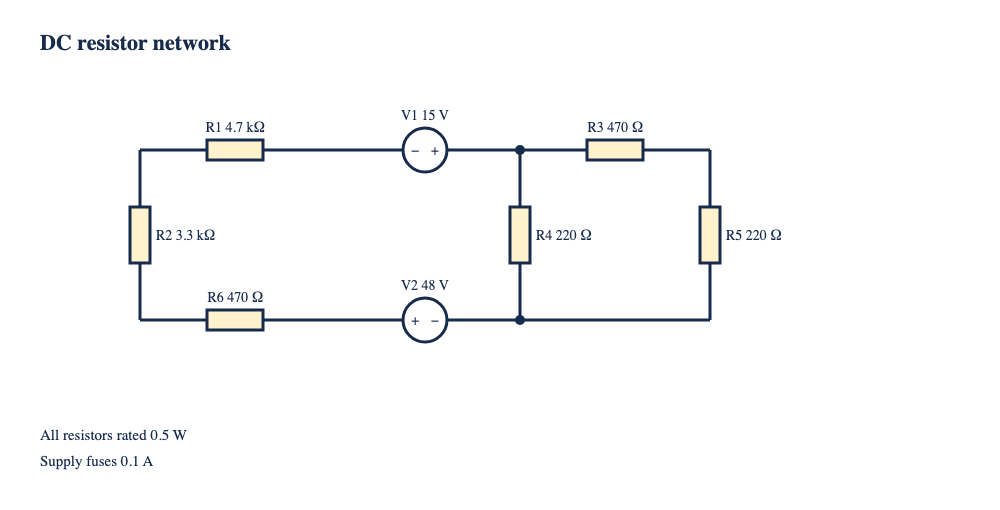
\includegraphics[width=\linewidth,trim=110 150 240 100,clip]{figures/teaser-dc_network-source.png}\\[-1pt]
{\footnotesize (a) Source drawing: \textbf{safe}}
\end{minipage}\hfill
\begin{minipage}[t]{.325\linewidth}\centering
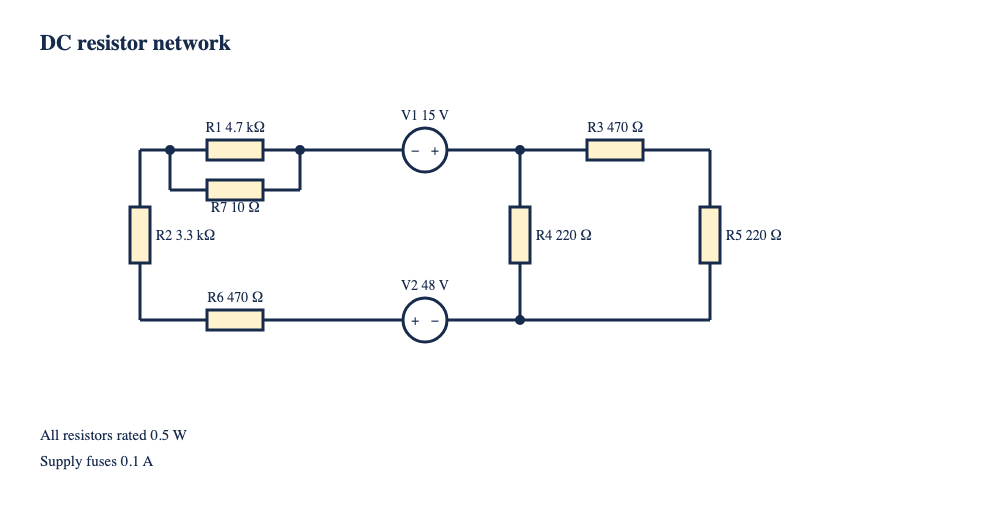
\includegraphics[width=\linewidth,trim=110 150 240 100,clip]{figures/teaser-dc_network-target.png}\\[-1pt]
{\footnotesize (b) ``Add R7 = 10\,$\Omega$ in parallel with R1.''}
\end{minipage}\hfill
\begin{minipage}[t]{.325\linewidth}\centering
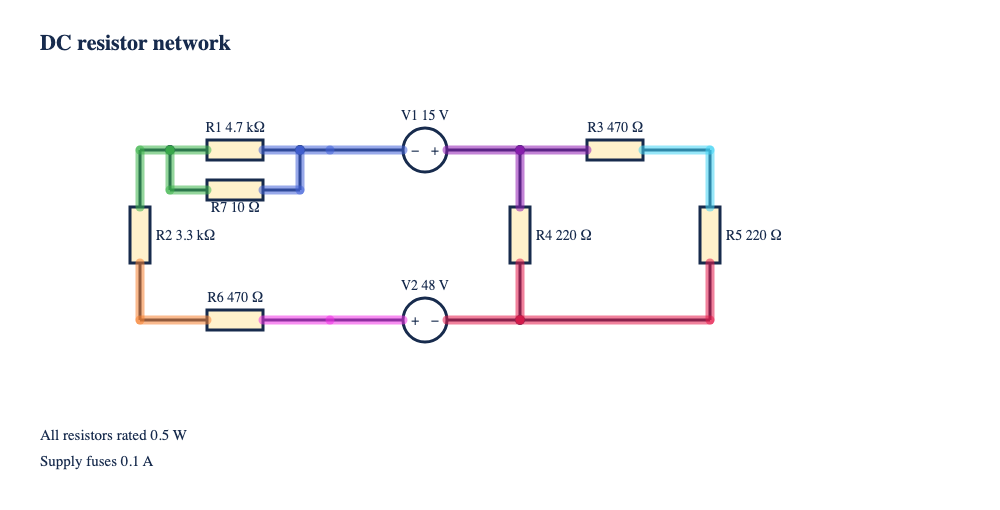
\includegraphics[width=\linewidth,trim=110 150 240 100,clip]{figures/teaser-dc_network-recovered.png}\\[-1pt]
{\footnotesize (c) Network recovered from (b): \textbf{unsafe}}
\end{minipage}
\captionsetup{hypcap=false}
\captionof{figure}{\textbf{Scoring an edit by re-solving the drawing.} A one-resistor edit to a two-source
network (a$\to$b) looks innocuous, but it overloads a component elsewhere in the circuit. \ours reads only
the visible SVG, rebuilding every electrical node from wire endpoints, T-junctions and junction dots (each
colour in (c) is one node), reading component values from their labels, and solving the network. Here the
edited drawing violates its own note: R2 now dissipates 0.84\,W against a 0.5\,W rating. The same procedure
scores any edited drawing, whoever or whatever produced it.}
\captionsetup{hypcap=true}
\label{fig:teaser}
\end{strip}

\begin{abstract}
Language models now create and edit engineering schematics directly as SVG, but current evaluations score
the markup or the pixels, not what the edited drawing means physically. We introduce \ours, a verifier that
reads a circuit or water-distribution drawing \emph{as built}. It recovers the network from visible geometry
and labels alone, respecting junction and crossing conventions, and re-solves it by nodal analysis or a
Newton flow--head solve cross-checked by Hardy Cross. It then grades an edit by whether the drawing describes the
intended network and whether that network meets the criteria printed on it. The verifier passes
\numControls{} analytical controls and recovers all \roundTripTotal{} of \roundTripTotal{} generated test
drawings exactly. It is invariant to identifiers, element order and scale. We release \netEdits{} physics-verified
text-guided edits and a harder evaluation tier with up to \hardMaxLoopsDC{} independent loops. Under this
grading, a frontier model (\astra) edits every completed task correctly and analyses circuits exactly, but
declares an unsafe pipe network safe without any sign of doubt. Replacing its analysis with a solve of its
own drawing removes that error. \abstractOurs
\end{abstract}

\section{Introduction}
\label{sec:intro}

Circuit schematics and water-network plans are routinely exchanged as vector drawings, and language models
are now asked to create and edit them directly as SVG markup. An edit that looks correct can still change the
physics. Adding a resistor in parallel with one component redistributes current through the whole network
(\cref{fig:teaser}); removing a pipe reroutes flow and can drop the pressure at a distant junction below its
service minimum. Whether an edit is acceptable is a property of the network the drawing \emph{describes},
not of its markup.

Existing evaluations do not measure that property. SVG-editing benchmarks compare the output with a
reference by markup or pixel similarity~\cite{svgeditbench,scidiagramedit}, which penalises harmless
re-formatting and cannot tell a correctly drawn but dangerous design from a safe one. Engineering-reasoning
benchmarks score numerical answers to problems stated in text or
code~\cite{feabench,fem_bench,pdeagent_bench}, not the drawing a model hands back. Between the two sits the
question an engineer actually asks of an edited schematic: \emph{if I read this drawing as built, what does it
do, and is it safe?}

We answer that question mechanically. \ours recovers the network from the visible SVG alone: wire and pipe
endpoints, T-junctions, junction dots, component symbols and their labels, read under standard drafting
conventions and with no access to identifiers or metadata. It then solves the recovered network by modified
nodal analysis for circuits and by a Newton solve of flows and heads for pipe networks, and compares the
solution with the intended design. Because the score depends only on the network, any drawing can be graded
the same way, whether it comes from a patch, a re-typed SVG or a human drafter.

\paragraph{Contributions.}
\begin{itemize}
\item \textbf{A drawing-grounded verifier} for resistor and water-distribution networks. It is invariant to
      identifiers, element order and uniform scaling, it respects crossing and junction conventions, and it is
      validated against \numControls{} analytical controls and \roundTripTotal{} generated drawings, every one of
      which recovers exactly to its source design (\cref{sec:method}).
\item \textbf{Two physics-verified edit datasets}: \netEdits{} text-guided edits over \netDesigns{} networks
      for training and evaluation, and a harder evaluation-only tier of \hardEdits{} edits on networks with up to
      \hardMaxLoopsDC{} independent loops. Every gold patch reproduces its target exactly, and every safety
      verdict is computed from the drawing (\cref{sec:data}).
\item \textbf{A measurement of a frontier model} (\astra) under this scoring. It edits every completed task
      correctly and analyses circuits exactly, but its rare analysis error is silent: it declares an unsafe pipe
      network safe (\cref{sec:experiments}).
\item \textbf{A small verified editor.} A 1.5B model emitting tree patches, paired with the verifier, is correct on all
      1{,}000 held-out edits and on \editOneFiveHard\,\% of larger, unseen networks, with exact verdicts. How the patch
      names elements decides the outcome. Addressing by document position reaches \editOneFivePosMain\,\%, while
      addressing by SVG identifier reaches 100\,\%.
\end{itemize}

\section{Related work}
\label{sec:related}

\paragraph{Vector graphics generation and editing.}
Learned SVG generators model paths and primitives directly~\cite{carlier2020deepsvg} or emit SVG code with a
language-model decoder~\cite{rodriguez2025starvector}. Instruction-based SVG editing is benchmarked by
comparing the edited result with a reference image or markup~\cite{svgeditbench}, and scientific-diagram work
learns edits from paper revisions~\cite{scidiagramedit} or targets structure-faithful
generation~\cite{sciforma}. These methods treat a drawing as an image or a document. We treat an engineering
drawing as a specification of a physical network and score it by what that network does.

\paragraph{CAD and engineering design.}
Generative CAD models produce parametric construction sequences~\cite{wu2021deepcad,khan2024text2cad}, and
agentic systems couple language models to simulators for mechanics~\cite{mechagents} and finite-element
analysis~\cite{all_fem,vfeagent}. Benchmarks such as FEABench~\cite{feabench}, FEM-Bench~\cite{fem_bench}
and PDEAgent-Bench~\cite{pdeagent_bench} evaluate the reasoning or code that sets up a simulation. Our
verifier instead reads a finished two-dimensional drawing and reconstructs the model it implies, so it can
audit the artefact a designer or a model actually delivers.

\paragraph{Network analysis.}
Modified nodal analysis~\cite{ho1975mna} is the standard formulation for linear circuits. Pipe networks are
classically solved by loop corrections~\cite{hardycross1936} or by the gradient method on flows and
heads~\cite{todini1988} that underlies EPANET~\cite{rossman2000epanet}; we use Churchill's friction
factor~\cite{churchill1977}, which is continuous from laminar through fully rough flow. None of this is new.
What is new is running these solvers on networks recovered from free-form drawings, and using them as the
metric for text-guided editing.

\section{Drawing-grounded verification}
\label{sec:method}

\begin{figure}[t]
\centering
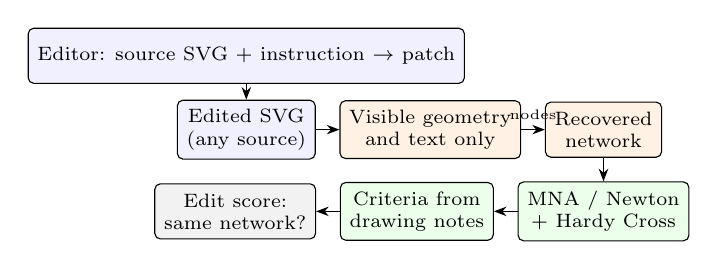
\begin{tikzpicture}[font=\scriptsize, node distance=3mm and 3mm,
  box/.style={draw, rounded corners=2pt, align=center, minimum height=7mm, fill=#1},
  box/.default={white}, >={Stealth[length=1.6mm]}]
\node[box=blue!6] (svg) {Edited SVG\\(any source)};
\node[box=orange!10, right=of svg] (geo) {Visible geometry\\and text only};
\node[box=orange!10, right=of geo] (net) {Recovered\\network};
\node[box=green!8, below=of net] (solve) {MNA / Newton\\$+$ Hardy Cross};
\node[box=green!8, left=of solve] (check) {Criteria from\\drawing notes};
\node[box=gray!10, left=of check] (score) {Edit score:\\same network?};
\draw[->] (svg) -- (geo);
\draw[->] (geo) -- node[above]{\tiny nodes} (net);
\draw[->] (net) -- (solve);
\draw[->] (solve) -- (check);
\draw[->] (check) -- (score);
\node[box=blue!6, above=2mm of svg] (editor) {Editor: source SVG $+$ instruction $\to$ patch};
\draw[->] (editor) -- (svg);
\end{tikzpicture}
\caption{\textbf{\ours.} Any edited drawing is read as built: geometry and labels become a network, the
network is solved, and the result is checked against the criteria printed on the drawing and compared with
the intended design. Identifiers and metadata are never read.}
\label{fig:pipeline}
\end{figure}

\paragraph{Task.} A source drawing $S$ of a network and an instruction $u$ (\eg ``Add R7 = 10\,$\Omega$ in
parallel with R1'') define a target design $D^\star$. An editor returns a drawing $\hat S$. We ask two
questions of $\hat S$: does it describe $D^\star$ (\emph{edit correctness}), and does the network it describes
satisfy the criteria stated on the drawing (\emph{verdict})? Both are decided by recovering a network
$\mathcal{R}(\hat S)$ from the drawing and solving it.

\subsection{Recovering a network from a drawing}
Recovery parses the SVG with transforms applied and rejects scripts, external references, clipping and
masking. It then reads only what is visibly drawn.

\paragraph{Connectivity.} Stroked straight segments are candidate conductors (for pipe networks, only heavy
strokes). A segment endpoint lying in the interior of another segment is a T-junction and splits it; a filled
junction dot splits every segment passing through its centre. Two segments that merely cross stay
unconnected, which is the drafting convention for both schematics and piping plans. Endpoints closer than
$\tau = 10^{-3}$ drawing units are merged. For circuits, all points joined by wire form one electrical node.
For pipe networks, nodes are points of degree $\neq 2$, dotted points and points on a reservoir outline, and
every chain of segments between two nodes is one pipe. A $90^\circ$ turn along a chain is an elbow; other
bend angles are rejected.

\paragraph{Components.} A rectangle whose two short-side midpoints coincide with conductor endpoints is a
resistor between the corresponding nodes. A circle is classified by where conductors meet it, not by its size:
if a conductor passes through its centre it is a junction dot, and if exactly two conductors end on its rim it
is a voltage source, whose positive terminal is the one nearer the ``$+$'' mark inside it. Filled rectangles
touched by pipe ends are reservoirs. Classifying by incidence rather than radius or stroke width keeps recovery
unchanged under uniform scaling of the drawing.

\paragraph{Values and criteria.} Labels are parsed with fixed grammars (\eg \code{R3 4.7 k$\Omega$},
\code{P5 320 m \O 150}, \code{J2 q=6 L/s z=10 m}) and assigned one-to-one to the nearest component or pipe,
within a reach proportional to the drawing's own scale (the median resistor body or pipe segment). Design
criteria are read from the drawing's notes: the resistor power rating and supply fuse; the pipe roughness,
elbow loss coefficient, minimum pressure head and maximum velocity. A drawing that leaves any component
unlabelled, or has two labels competing for one component, is reported as unreadable rather than guessed at.

\subsection{Solving the recovered network}
\paragraph{Circuits.} We use modified nodal analysis~\cite{ho1975mna} with one grounded node per connected
part of the network, so a floating fragment carries no current and does not make the system singular. A source
whose terminals share a node, or a loop made only of sources, makes the system singular; such a drawing is
reported as ill-posed. The outputs are every branch current, every resistor's dissipation and every source's
current; the criteria are $P_R \le P_\text{rated}$ for each resistor and $|I_V| \le I_\text{fuse}$ for each
source.

\paragraph{Pipe networks.} For pipe $p$ from node $a$ to node $b$ with flow $Q_p$, the head loss is
\begin{equation}
h_p(Q_p) = \Big(f(\mathrm{Re}_p,\varepsilon/D_p)\,\frac{L_p}{D_p} + n_p K_\text{elbow}\Big)
\frac{v_p |v_p|}{2g},
\end{equation}
where $v_p = 4Q_p/(\pi D_p^2)$, $f$ is Churchill's friction factor~\cite{churchill1977} and $n_p$ is the number
of elbows counted from the drawing. We solve jointly for pipe flows and junction heads,
\begin{equation}
h_p(Q_p) = H_a - H_b \;\;\forall p, \qquad
\textstyle\sum_{\text{in}} Q_p - \sum_{\text{out}} Q_p = q_j \;\;\forall j,
\end{equation}
with reservoir heads fixed, by Newton's method with backtracking~\cite{todini1988}, stopping at residuals below
$10^{-10}$\,m and $10^{-13}$\,m$^3$/s. Because Churchill's $f$ tends to $64/\mathrm{Re}$ in laminar flow, $h_p$
has a finite, non-zero slope at $Q_p = 0$ and the Jacobian stays regular when a flow reverses. As an independent
check, every network is also solved by Hardy Cross loop corrections~\cite{hardycross1936}, with multiple
reservoirs joined through a virtual datum node. The criteria are $|v_p| \le v_\text{max}$ for each pipe and
$H_j - z_j \ge p_\text{min}$ for each junction.

\subsection{Scoring an edited drawing}
An edit is \emph{correct} when $\mathcal{R}(\hat S)$ equals the target network $D^\star$ in two senses. The
first is topological: we compare, for every node, the multiset of named component terminals it touches, which
is a complete invariant of a network with named components, together with every component value and every
criterion. The second is physical: the two solutions agree, with currents within $10^{-9}$ relative plus
1\,pA, flows within $10^{-9}$\,m$^3$/s and heads within $10^{-7}$\,m. Markup is irrelevant: a drawing that
re-orders elements, renames identifiers or re-formats numbers is credited if it describes the same network,
and a drawing that is byte-for-byte plausible but disconnects a wire by $0.01$ units is not.

\subsection{Validating the verifier}
\label{sec:validation}
\Cref{tab:controls} lists the analytical controls. They include a balanced and an unbalanced Wheatstone
bridge; we initially chose bridge values that happened to balance, which made the ``unbalanced'' control
vacuous and hid a sign error, and we record this as a caution. Beyond the controls, \roundTripTotal{}
independently generated drawings (source designs and all their edits, over two seeds) recover to exactly
the network they were drawn from, as do all \datasetDrawings{} drawings in the released datasets.
Unit tests confirm four further properties: recovery is unchanged by stripping identifiers, shuffling
elements, translating and uniformly scaling the drawing by $\times0.25$ to $\times4$; a T-junction joins,
while a crossing joins only when dotted; moving only the ``$+$'' mark reverses every branch current; and moving
one wire endpoint by $0.01$ units breaks the connection. Two of these tests found real defects in the first
version. A fixed-radius rule for junction dots misclassified dots once the drawing was scaled up, and an
absolute current tolerance misjudged an edit whose two sources exactly cancel.

\begin{table}[t]
\centering
\footnotesize
\setlength{\tabcolsep}{3pt}
\begin{tabular}{@{}p{4.55cm}rr@{}}
\toprule
Control & \ours & Reference \\
\midrule
\controlRows
\bottomrule
\end{tabular}
\caption{\textbf{Analytical controls} for the two solvers. References are closed forms, an independent
bisection, or a second algorithm.}
\label{tab:controls}
\end{table}

\section{Datasets}
\label{sec:data}

\paragraph{Resistor networks.} A design starts from a grid of $2$--$3 \times 3$--$5$ nodes. Edges are removed
at random while the graph stays connected and bridgeless (a bridge would carry no current), until $2$--$6$
independent cycles remain. Each edge becomes a resistor (E6 series, 10\,$\Omega$--6.8\,k$\Omega$), a plain wire
(20\,\%), or one of one or two DC sources (5--48\,V, random polarity). Designs are rejected if a resistor is
shorted, if sources form a loop, or if no current flows. Notes state a resistor power rating (0.25--2\,W) and a
supply fuse (0.1--1\,A). Drawings use standard symbols, with junction dots at nodes of degree three or more.

\paragraph{Water-distribution networks.} A random spanning tree of a $2$--$3 \times 3$--$5$ grid receives one to
three extra pipes to close loops. Some dead ends are pruned, and one or two reservoirs attach at the boundary.
Grid points of degree $\neq 2$, plus about a third of the rest, become junctions carrying a demand
(0--15\,L/s) and an elevation (0--30\,m). The remaining pass-through points become straight runs or
$90^\circ$ elbows. Pipes have lengths of 100--800\,m and nominal diameters of 80--300\,mm, and notes state the
roughness, elbow loss coefficient ($K=0.9$), minimum pressure head (10--20\,m) and maximum velocity
(1.5--2.5\,m/s).

\paragraph{Edits.} Each design receives four instructions. For circuits these are a resistor value change, a
source voltage change, a polarity reversal (two-source designs) or opening a branch (one-source designs,
provided the network stays solvable), and adding a resistor in parallel with an existing one, drawn as a
tapped branch. For pipe networks they are a diameter change, a demand change, removing a pipe (provided every
junction stays supplied and no reservoir is cut off), and adding a pipe between adjacent junctions (or, if
none exist, a length change). Target drawings are rendered from the edited design. The gold edit is a tree patch
derived between source and target SVG, applied with a validating executor and required to reproduce the
target exactly. A row is kept only if both drawings recover to their designs and, for pipes, Newton and Hardy
Cross agree to $10^{-9}$\,m$^3$/s.

\paragraph{Statistics.} \Cref{tab:data} summarises both tiers. The \emph{hard} tier uses $4$--$5 \times
5$--$6$ grids with $8$--$16$ independent loops for circuits and four to eight added pipes for water networks.
It is evaluation-only: no model is trained on networks of that size. Splits are by source design, so the four
edits of one drawing never cross splits.

\begin{table}[t]
\centering
\footnotesize
\setlength{\tabcolsep}{3.2pt}
\begin{tabular}{lrr}
\toprule
 & Main (v1) & Hard \\
\midrule
\dataRows
\bottomrule
\end{tabular}
\caption{\textbf{Datasets.} Loops are independent cycles of the recovered network (median, range). ``Verdict
flips'' are edits that turn a safe design unsafe or the reverse. All patches reproduce their targets and all
drawings recover to their designs.}
\label{tab:data}
\end{table}

\section{Experiments}
\label{sec:experiments}

\paragraph{Frontier model.} We evaluate \astra (\code{gpt-6-astra}) through the Chat Completions API at medium
reasoning effort, with a 32{,}000-token completion cap, no tools, \code{store=false} and one sample per task.
\astra works in its natural mode: it receives the drafting conventions, the physical model (fluid properties,
friction law, loss conventions) and the criteria in the prompt, and it returns the complete edited SVG followed
by a JSON analysis stating the verdict, the violating components and the governing quantities. The edited SVG
is scored by \ours exactly as any other drawing (\cref{sec:method}), and the analysis is compared with the
solver's. Tasks are the first ten test edits by identifier for every (family, edit type) pair of the main tier
(100 tasks), and the first four of the hard tier (40 tasks). The API account ran out of credit during the run.
All \astraMainN{} main-tier and \astraHardN{} hard-tier tasks that completed are reported. Every circuit task
completed. The missing tasks are all pipe networks, which failed with ``no credits remaining'' (26) or a
dropped connection (12), and they are excluded rather than counted as failures.

\paragraph{Our editor.} \ours pairs the verifier with a small editor: Qwen2.5-Coder-Instruct~\cite{hui2024qwen25coder}
at 1.5B and 7B parameters, fine-tuned with LoRA~\cite{hu2022lora} (rank 16 on the attention projections) for two
epochs on the \netEdits{}-edit training split to map \emph{source SVG $+$ instruction} to a tree patch. The patch
is applied by a validating executor, and the resulting drawing is recovered and solved, so the verdict is
computed, not generated. Decoding is greedy. The hard tier is never seen in training.

\paragraph{Metrics.} \emph{Edit}: the edited drawing recovers to the target network. \emph{Verdict}: the stated
pass/fail matches the solver's. \emph{Violations}: the set of violating components matches exactly. \emph{All}: all
three at once. For systems whose verdict is computed by \ours, the verdict is taken from the solve of the edited
drawing, whether or not the edit was correct.

\begin{table*}[t]
\centering
\footnotesize
\setlength{\tabcolsep}{5pt}
\begin{tabular}{lcccc}
\toprule
System & Edit & Verdict & Violations & All \\
\midrule
\multicolumn{5}{l}{\textbf{Main tier} (same completed tasks for every system)} \\
\compareMainRows
\midrule
\multicolumn{5}{l}{\textbf{Hard tier} (8--16 loops for circuits; unseen in training)} \\
\compareHardRows
\bottomrule
\end{tabular}
\caption{\textbf{Edit and verdict accuracy}, \% (count), on the tasks \astra completed. ``\astra drawing $+$
\ours verdict'' keeps \astra's edited SVG but replaces its analysis with the solve of that drawing.}
\label{tab:compare}
\end{table*}

\subsection{What \astra gets right}
\astra is an accurate editor of these drawings. Every one of its completed edits recovers to the target
network, including parallel branches drawn as tapped sub-circuits and pipes added between junctions, and it
never disconnected a wire or broke the drafting conventions. Its circuit analysis is exact on every
completed task, including hard-tier networks with up to 16 independent loops. We did not find the failure
boundary we expected for linear networks: at these sizes, unaided nodal analysis is within reach. Each answer
costs \$\astraMainCost{} on the main tier and \$\astraHardCost{} on the hard tier on average, and takes a median
of \astraMainSeconds{}\,s and \astraHardSeconds{}\,s respectively, with no truncated responses.

\subsection{Where it fails: silently}
\begin{figure}[t]
\centering
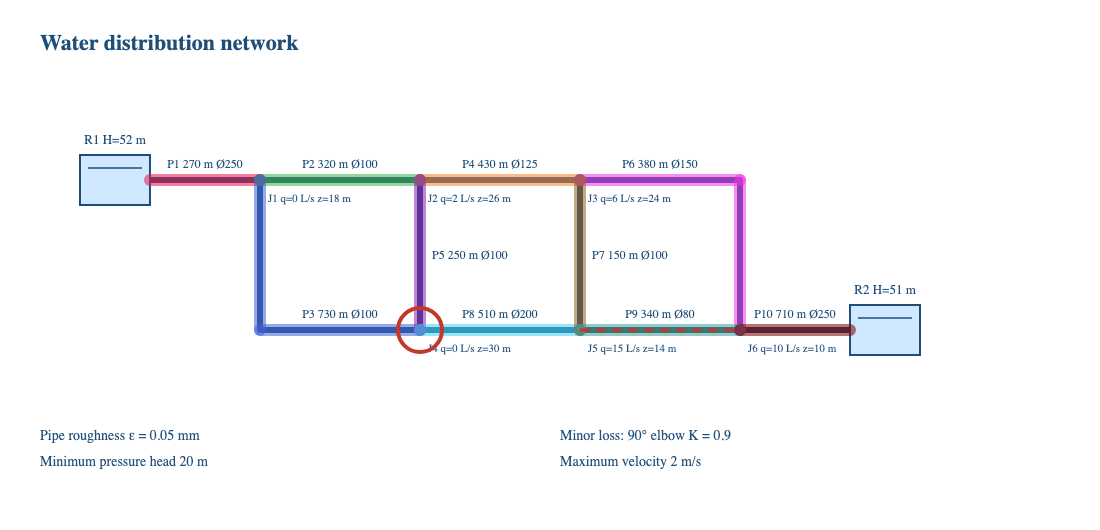
\includegraphics[width=\linewidth,trim=60 150 160 120,clip]{figures/astra-failure-pipe.png}
\caption{\textbf{A confident wrong verdict.} ``Change the length of P9 to 340\,m'' (dashed) in a two-reservoir
network with four loops. \astra's edit is correct, and it reports the minimum pressure head at J4 (circled) as
20.04\,m and the design as passing. Re-solving the drawing gives 19.23\,m, below the 20\,m minimum stated on
the drawing. Several of its pipe velocities are off by up to 67\,\%.}
\label{fig:failure}
\end{figure}

The only substantive error among \astra's completed answers is in a nonlinear pipe network, and it is not flagged
(\cref{fig:failure}). The edit is right, but the analysis declares a failing design safe: it reports 20.04\,m
of pressure head where the drawing yields 19.23\,m against a 20\,m minimum, and its flows are wrong
throughout the loop that contains the edited pipe. Nothing in the answer
distinguishes it from the correct ones: it finished normally, used a similar reasoning budget, and presented
its numbers with the same precision. This is the failure mode a verifier exists for. It is rare (1 of
\astraMainN{} main-tier answers), it concentrates where the physics is nonlinear and the design sits near a
limit, and it cannot be detected from the answer itself. Replacing \astra's analysis with the solve of its
own drawing removes it (\cref{tab:compare}, second row).

\subsection{The small editor}
\oursDiscussion

\begin{table}[t]
\centering
\footnotesize
\setlength{\tabcolsep}{3pt}
\begin{tabular}{lccc}
\toprule
\ours editor & Edit (circuits) & Edit (pipes) & All \\
\midrule
\oursFullRows
\bottomrule
\end{tabular}
\caption{\textbf{Our editor on the full test sets}: 1{,}000 main-tier and \hardEdits{} hard-tier edits.}
\label{tab:ours}
\end{table}

\subsection{Cost of a verified edit}
\costDiscussion

\section{Limitations and conclusion}
\label{sec:conclusion}

\paragraph{Limitations.} The networks are procedural: rectilinear layouts, a fixed symbol vocabulary and
label grammar, steady DC circuits with ideal sources, and steady incompressible pipe flow with elbow losses
only. Recovery is strict by design. A drawing that uses other symbols, draws a resistor as a zig-zag, or
places labels far from their components is reported as unreadable, not interpreted. The frontier-model
study covers one model at one reasoning effort with one sample per task, and its pipe-network arm is
incomplete because the API account ran out of credit, so the hard pipe tier in particular is under-measured.
The single wrong verdict is a demonstrated failure mode, not an estimated rate. The numerical tolerance for
\astra's reported velocities gained an absolute floor of 0.01\,m/s after we saw that three-decimal rounding of
near-zero velocities was being scored as error. Verdicts and edits are unaffected by this change.

\paragraph{Conclusion.} An edited engineering drawing can be graded by reading it as built and solving what it
describes. This removes the dependence on markup that makes current SVG-editing metrics fragile, and it turns
``is this edit safe?'' into a computation instead of a claim. Under that grading a frontier model is a
strong editor and usually a strong analyst, but its rare analysis errors are silent. Pairing any editor with a
drawing-grounded solve makes the verdict exact whenever the edit is right.
\conclusionOurs


{
    \small
    \bibliographystyle{ieeenat_fullname}
    \bibliography{refs}
}

\clearpage
\appendix
\section{Supplementary material}
\subsection{Prompt given to \astra}
System message:
\begin{lstlisting}
You are an engineering drafting and analysis assistant. Use your own reasoning; no external tools are provided. Do not claim you ran a solver.
\end{lstlisting}
User message for a circuit task, verbatim up to the source SVG, which follows in full:
\begin{lstlisting}
Instruction: Set R3 to 150 Ω.

Drawing conventions: straight lines are ideal wires. A wire that ends on another wire (a T) is connected to it; a filled dot also marks a connection; wires that cross without a dot are NOT connected. Rectangles are resistors and circles are ideal DC voltage sources; the '+' inside a source marks its positive terminal. Labels give component names and values.
Criteria (from the drawing notes): every resistor's dissipated power must not exceed the stated rating, and the magnitude of every source's current must not exceed the stated supply fuse rating.

Tasks:
1. Apply the instruction to the drawing, changing nothing else, and return the complete edited SVG.
2. Analyse the EDITED design and report whether it meets every criterion.

Answer with exactly two fenced blocks and nothing else: first ```svg containing the full edited SVG, then ```json containing {"verdict": "pass" or "fail", "violations": [names of every resistor or source that violates a criterion], "source_currents_A": {"V1": current delivered out of its + terminal, ...}, "max_resistor_power_W": {"name": "R?", "value": watts}}

Source SVG:
[complete source SVG]
\end{lstlisting}
For pipe networks the conventions paragraph and the JSON schema are replaced by:
\begin{lstlisting}
Drawing conventions: heavy lines are pipes; filled dots are junctions. A pipe runs between junctions or reservoirs and may turn through 90-degree elbows; each elbow adds the minor-loss coefficient K given in the notes. 'P# L m ØD' gives a pipe's length (m) and internal diameter (mm); 'J# q=.. L/s z=.. m' gives the demand withdrawn at a junction and its elevation; 'R# H=.. m' is a reservoir's fixed total head.
Analysis model: steady incompressible water, density 998 kg/m3, dynamic viscosity 1.002e-3 Pa s, g = 9.80665 m/s2; Darcy-Weisbach head loss with the Churchill (1977) friction factor and the pipe roughness in the notes; tee and junction losses neglected; pressure head at a junction = hydraulic head minus elevation.
Criteria (from the drawing notes): every pipe velocity must not exceed the maximum velocity, and every junction pressure head must be at least the minimum pressure head.

JSON schema: {"verdict": "pass" or "fail", "violations": [names of every pipe or junction that violates a criterion], "pipe_velocities_m_s": {"P1": speed, ...}, "min_pressure_head_m": {"name": "J?", "value": metres}}
\end{lstlisting}

\subsection{Results by edit type}
\Cref{tab:kinds} breaks end-to-end accuracy down by edit type. The one type on which \astra is below 100\,\%
is the pipe-length change that produced its silent wrong verdict (\cref{fig:failure}). Positional addressing
fails mostly on circuit edits, and id addressing is correct on every main-tier type at both model sizes.
\begin{table*}[t]
\centering
\footnotesize
\setlength{\tabcolsep}{5pt}
\begin{tabular}{@{}lcccc@{}}
\toprule
Edit type & \astra & 1.5B pos. & 1.5B id & 7B id \\
\midrule
\kindRows
\bottomrule
\end{tabular}
\caption{End-to-end accuracy (edit, verdict and violations all correct), \% (count). \astra on its completed main-tier tasks; \ours editors (positional or id addressing) on the full 1{,}000-edit main test set.}
\label{tab:kinds}
\end{table*}

\subsection{Training stability}
The first 7B training run, on an H100 NVL, diverged: the loss rose from 0.65 at step 20 to $3.0{\times}10^{4}$
at step 30 with a non-finite gradient norm, and the resulting adapter emits only ``\texttt{!}'' characters. Two
50-step reruns with identical code, settings and data order isolate the cause to PyTorch's cuDNN kernel for
scaled dot-product attention. With it enabled the gradient norm again became non-finite at step 30. With it disabled
all 50 steps were finite and the loss fell from 0.55 to 0.026. The reported 7B editor was retrained with that kernel
disabled. The 1.5B editors, trained on an RTX PRO 6000, never used it. The diverged run is retained,
marked void, and excluded from every table, and the trainer now stops at the first non-finite loss or gradient.


\end{document}
